\documentclass[a4paper,12pt]{article}
\usepackage{graphicx}
\usepackage{titlesec}
\usepackage[utf8]{inputenc}
\usepackage{xcolor}
\usepackage{fancyhdr}
\usepackage{lipsum}
\usepackage{caption}

\renewcommand{\headrulewidth}{0pt}
\fancyhead[C]{}
\fancyhead[C]{
	
\includegraphics[width=4cm]{metu}
}
\pagestyle{plain}

%opening
\title{Middle East Technical University\\Department of Physics\\\textbf{PHYS307 Applied Modern Physics}}
\author{Oğuzhan ÖZCAN\\1852334}
\date{}
\clearpage
\thispagestyle{empty}
\providecommand{\groupmember}[1]{\textbf{Group Members:} }
\providecommand{\expdate}[1]{\textbf{Experiment Date:} }
\providecommand{\repdate}[1]{\textbf{Report Submit Date:} }
\providecommand{\expname}[1]{\textbf{Exp. MP-CE The Compton Effect} }


\usepackage[a4paper,%
left=0.5in,right=0.5in,top=0.5in,bottom=0.8in,%
footskip=.25in]{geometry}
%\topmargin -4.5cm
%\oddsidemargin 0.2cm
%\textwidth 16cm %
%\textheight 21cm%
%\footskip 1.0cm%




\begin{document}
\pagenumbering{gobble}
\maketitle

\thispagestyle{fancy}

%%%%%%%%%%%%%%%%%%%%%%%%%%%%%%%%%%%%%%%%%%%%%%%%%%%%%
\noindent\rule{18.4cm}{0.8pt}
\begin{center}
	\expname{arg1}{}
\end{center}
\groupmember{arg1}{Cem MADEN, İrem KÜL, Deniz AKYÜREK}\\

\noindent\rule{18.4cm}{0.8pt}\\\\
%%%%%%%%%%%%%%%%%%%%%%%%%%%%%%%%%%%%%%%%%%%%%%%%%%%%%
\begin{table}[h!]
\begin{center}
	\begin{tabular}{|p{3cm}|p{3cm}|p{3cm}|p{3cm}|}
	\hline Scattering Angle & Energy of the Scattered Photon [keV] & Wavelength of the Scattered Photon [m] & Compton Wavelength [m] \\ 
	\hline 30$^{\circ}$ & 538.5 & 2.30$\times10^{-12}$ & 3.69$\times10^{-13}$ \\ 
	\hline 
\end{tabular}
\caption{Energy and wavelength of the scattered photon} 
\end{center}
\end{table}

Experimentally found mean and standard deviation of Compton Wavelength = 0.369 pm\\
Expected value of the Compton Wavelength = 2.36 $\pm $ 0.14 pm\\\\
\textbf{1. Explain. Why are there relatively many counts at energies less than the energy of the incident photons in both spectra obtained by the use of two Cs$^{137}$ source with different activities.}\\\\
It is because we did not calibrate the experiment setup.\\\\
\textbf{2. Explain. Why are there relatively many counts at energies less than the energy of the expected scattered photons.}\\\\
There was background radiation which is caused by other radioactive elements on in the laboratory, cosmic rays and used radiation source Cs-137 in the experiment. Another cause is that when a $\gamma$-photon enters it scatters several times. After each scattering photon loses some energy and a free electron is produced. \\\\
\textbf{3. In a Compton scattering an electron is accelerated straight ahead in the same direction as that of the incident $\gamma$-ray photon. Which way does the scattered photon move?}\\\\
Momentum conservation requires that the total initial momentum be equal to the total final momentum. The total initial momentum consists only of the forward momentum of the incoming photon. Therefore, the direction of the final total momentum of the recoiling electron and the scattered photon must point in the +x direction.  There can be no component of the final total momentum along the +y or –y direction. Thus, in order for the y component of the total final momentum to be absent, the scattered photon must move either in the +x or –x direction.\\\\
\textbf{4. A photon can undergo Compton scattering from a molecule such as nitrogen, just as it does from an electron. However, the change in photon wavelength is much less than when the scattering is from an electron. Explain why?}\\\\
To see why, let examine below equation which gives the difference between the wavelength $\lambda^{\prime}$ of the scattered photon and the wavelength $\lambda$ of the incident photon in terms of the scattering angle $\theta$. 
\begin{equation}
\lambda^{\prime}-\lambda=[h/(mc)](1-\cos \theta)
\end{equation}
The mass of a nitrogen molecule is much greater than the mass of an electron.  Therefore, the factor $h/mc$ will be much smaller if the target particle is a nitrogen molecule.  Consequently, the change in the photon wavelength, $\lambda^{\prime}-\lambda$ is much less than it is when the target particle is an electron.\\\\
\textbf{5. In a specific experiment 500 keV energetic $\gamma$-rays are required but unfortunately there is only a Cs$^{137}$ source in the laboratory. How would you manage to convert the gamma photon from Cs$^{137}$ to 500 keV photons?}\\\\
If photons are Compton scattered, we can have 500 keV photons. For this value we have to determine the angle of scattering by using following calculation\\
Wavelength of 500 keV photons
\begin{equation}
\lambda=\frac{hc}{E}=\frac{(4.135\times 10^{-15} eV\cdot s)\cdot 3.0\times 10^{8}m/s}{500\times 10^{3} eV}=2.481\times 10^{-12} m
\end{equation}
Angle of scattering will be
\begin{equation}
\theta = \cos ^{-1}(1-\frac{\Delta \lambda }{\wedge})
\end{equation}
where
\begin{equation}
\Delta \lambda = 2.481\times 10^{-12}-1.873\times 10^{-12}=6.08\times 10^{-13} m
\end{equation} 
and $\wedge=2.36\times 10^{-13} m$. Therefore, angle of scattering will be
\begin{equation}
\theta = \cos ^{-1}(1-\frac{6.08\times 10^{-13} m}{2.36\times 10^{-13} m})=\cos ^{-1}(0.743)=42^{\circ}
\end{equation}
If we scatter photon with an angle of $42^{\circ}$, we get 500 keV photons.\\\\
\textbf{6. Must Compton scattering take place only between X- or $\gamma$-rays and free electrons? Can blue light undergo Compton scattering with a free electron?}\\\\
The wavelength of blue light is varies between 450 nm to 495 nm which is much larger than the Compton wavelength of the electron. For visible light, the Compton
shift is negligibly small compared with its wavelength. So the change in wavelength of
the visible light due to the Compton scattering would be too small to be measured.
\newpage
\textbf{Discussion and Conclusion}\\\\
This experiment shows a crucial topic in Physics which is Compton effect. Normally, we must took data between 0 and 90 degree but we only measured the angle of 30 degree. That is why we could not compare experimental data whether it is decreases or increases due to increasing in angle. Since we have only one data, we cannot calculate a standard deviation error. However, we can calculate a percentage error. At 30$^{\circ}$, energy of a scattered photon 564 keV [1]. Therefore
\begin{equation}
Percentage Error=\frac{|Theoretical Value-Experimental Value|}{Theoretical Value}\times 100
\end{equation} 
\begin{equation}
Percentage Error=\frac{|564-538.5|}{564}\times 100 = 4.52 \%
\end{equation}
As we can see, we have very low percentage error. It is because, we measured this data in 300 seconds. In the lab, we set two different point for measurement. We had some background reading while taking data it is because our radiation source was radiating at all angles. We have seen a graph like below
\begin{figure}[h!]
\centering
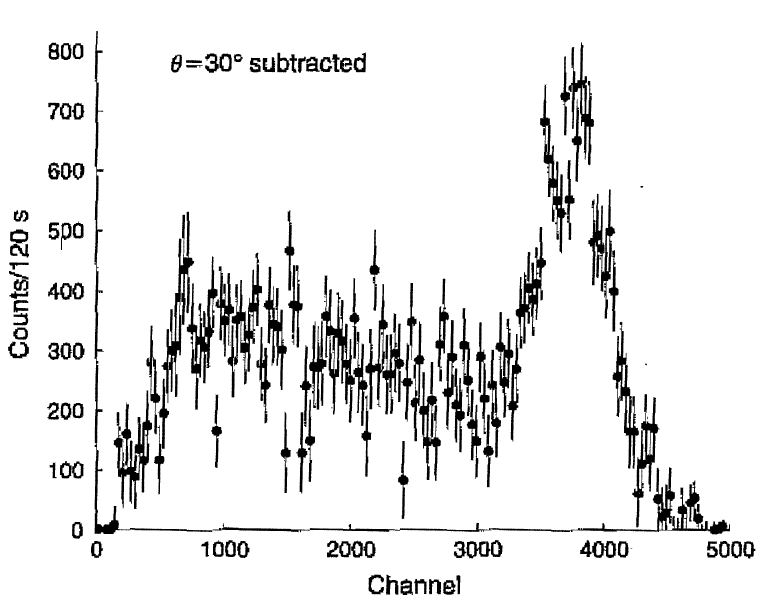
\includegraphics[scale=0.7]{Capture}
\caption{Plot of $\gamma$-rays at 30$^{\circ}$ for 120 secs}
\label{fig:Capture}
\end{figure}
All in all, we can say that this experiment is successful. We have very low percentage error which caused probably by instrumentation error.\\\\
\textbf{References}\\\\
$[1]$ Melissinos, Adrian C. \textit{Experiments in Modern Physics},. New York: Academic Press, 1966. 382.














































































































































\end{document}
